\documentclass[conference]{IEEEtran}
\IEEEoverridecommandlockouts
% The preceding line is only needed to identify funding in the first footnote. If that is unneeded, please comment it out.
\usepackage{cite}
\usepackage{amsmath,amssymb,amsfonts}
\usepackage{algorithmic}
\usepackage{graphicx}
\usepackage{textcomp}
\usepackage{xcolor}
\usepackage{siunitx}
\def\BibTeX{{\rm B\kern-.05em{\sc i\kern-.025em b}\kern-.08em
    T\kern-.1667em\lower.7ex\hbox{E}\kern-.125emX}}
\begin{document}

\title{Design and Simulation of a 3-bit R-2R DAC based on a 5-Transistor OTA in 180nm CMOS Technology\\
}

\author{\IEEEauthorblockN{ Bai Jia Qi}
\IEEEauthorblockA{\textit{Shanghaitech University} \\
baijq2024@shanghaitech.edu.cn 2024531050}

}

\maketitle

\begin{abstract}
This report details the design, implementation, and analysis of a 3-bit Digital-to-Analog Converter (DAC) based on the R-2R ladder architecture. The primary objective was to translate a 3-bit digital input code into a corresponding analog voltage with high linearity, characterized by minimal Differential Nonlinearity (DNL) and Integral Nonlinearity (INL) errors.
\end{abstract}

\begin{IEEEkeywords}
Operational transconductance amplifier, R-2R ladde, Resistor network, Signal Processing.
\end{IEEEkeywords}

\section{Introduction}
Digital-to-Analog Converters (DACs) are essential components in mixed-signal systems, converting digital signals into analog voltages for applications such as audio processing and communications. The R-2R ladder architecture is widely used due to its simple structure requiring only two resistor values, which benefits component matching and integrated circuit implementation. The five-transistor Operational Transconductance Amplifier (OTA) serves as a compact and effective solution for the required current-to-voltage conversion.

This paper presents the design of a 3-bit R-2R DAC with a focus on achieving high linearity, as measured by Differential Nonlinearity (DNL) and Integral Nonlinearity (INL). Section II details the design and analysis of the five-transistor OTA. Section III describes the complete DAC system and evaluates its performance. The paper concludes with a summary of the key results.

\section{FIVE-TRANSISTOR OTA DESIGN}

\subsection{The structure}

\begin{figure}[htbp]
\centerline{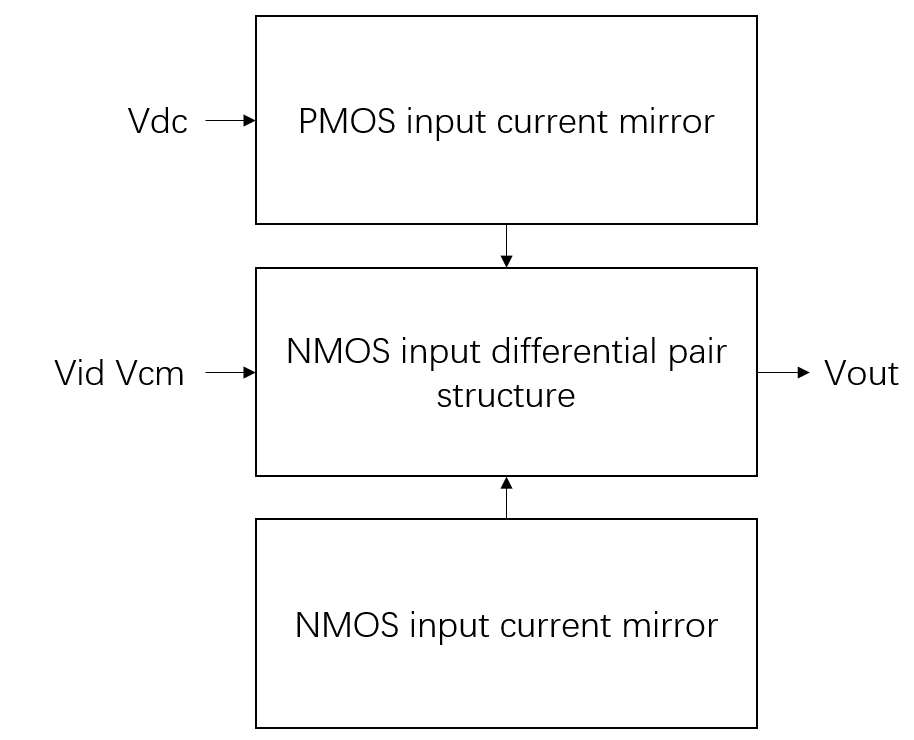
\includegraphics[width=0.3\textwidth]{figurestru1.png}}
\caption{Schematic of the 5-transistor OTA topology}
\label{fig}
\end{figure}

It converts differential input voltage into a single-ended output current.And it consists three parts, which are NMOS Differential Pair, PMOS Current Mirror Load and NMOS Tail Current Source.

\subsubsection{NMOS Differential Pair}
The NMOS differential pair forms the input stage and represents the core of the OTA. It consists of two perfectly matched NMOS transistors whose primary function is to convert a differential voltage into a differential current. 

\subsubsection{PMOS Current Mirror Load}
The PMOS current mirror load, comprising matched PMOS transistors, acts as an active load performing two critical functions. First, it converts the two complementary output currents from the differential pair into a single-ended output signal. Second, it provides high impedance at the output node, which is essential for achieving substantial voltage gain.

The voltage gain ($A_v$) can be approximated as:
\begin{equation}
A_v = g_m \cdot R_{out}
\end{equation}
where $R_{out}$ represents the high output impedance provided by this stage.

\subsubsection{NMOS Tail Current Source}
The NMOS tail current source provides stable, constant current biasing for the entire differential pair. This component sets the OTA's operating point. Crucially, its high output impedance significantly enhances the circuit's Common-Mode Rejection Ratio, enabling effective rejection of noise or interference common to both inputs.


\subsection{Circuit Implementation}

The NMOS and PMOS transistors in the circuit are the TSMC180nmN and TSMC180nmP models, respectively. In our design process, we aim to bias each MOSFET at \(V_{GS} = 0.6\ \mathrm{V}\) and \(V_{DS} = 0.6\ \mathrm{V}\), with a drain current \(I_D\) of either \(10\ \mathrm{\mu A}\) or \(20\ \mathrm{\mu A}\). We need to design the width (\(W\)) and length (\(L\)) accordingly. Suitable values for \(W\) and \(L\) are determined through DC sweep analysis.
The NMOS transistor with a $W/L$ ratio of 3 conducts a drain-source current ($I_{DS}$) of $10\ \mathrm{\mu A}$ when biased at a gate-source voltage ($V_{GS}$) of $0.6\ \mathrm{V}$.And the one with a $W/L$ ratio of 6 conducts a drain-source current ($I_{DS}$) of $20\ \mathrm{\mu A}$.Under same circumstance a PMOS with a $W/L$ ratio of 12 conducts a drain-source current ($I_{DS}$) of $10\ \mathrm{\mu A}$.
We use these three types of MOSFET to compose the circuit.

\begin{figure}[htbp]
\centerline{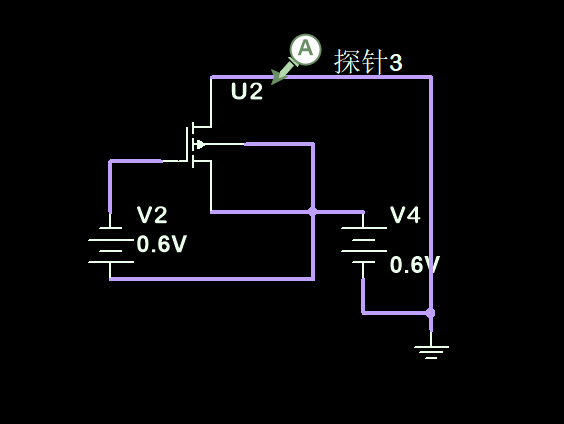
\includegraphics[width=0.35\textwidth]{single.png}}
\caption{Test circuit for characterizing the PMOS transistor}
\label{fig}
\end{figure}

We obtained the results:
\begin{figure}[htbp]
\centerline{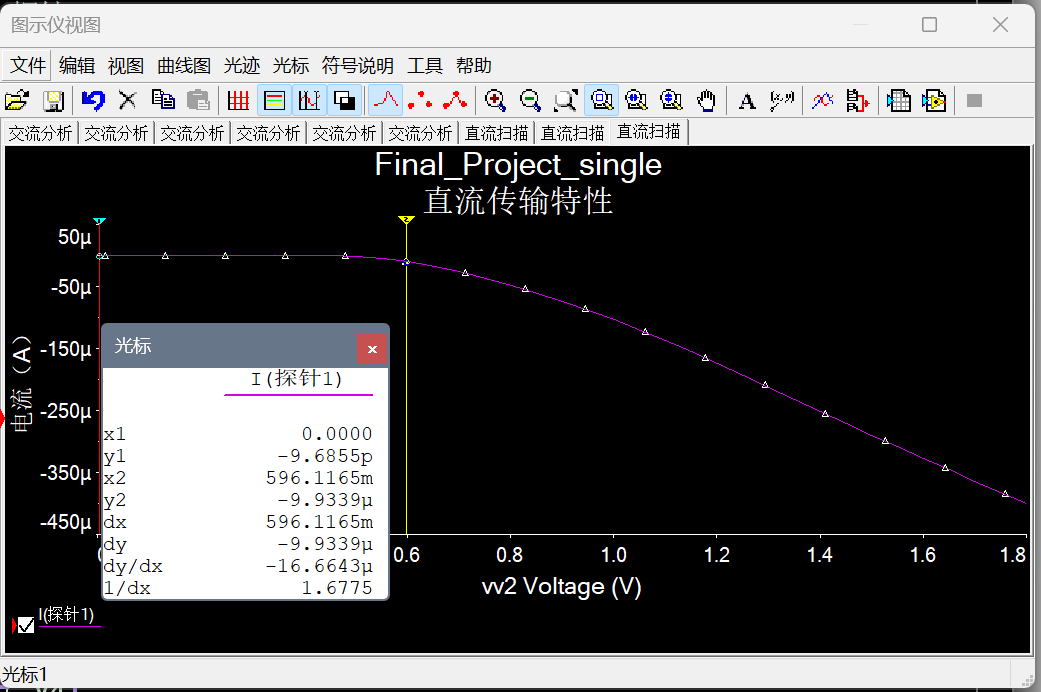
\includegraphics[width=0.35\textwidth]{NMOS_1_3_0.6V_10uA.png}}
\caption{I-V curve of NMOS with W/L=3 }
\label{fig}
\end{figure}


\begin{figure}[htbp]
\centerline{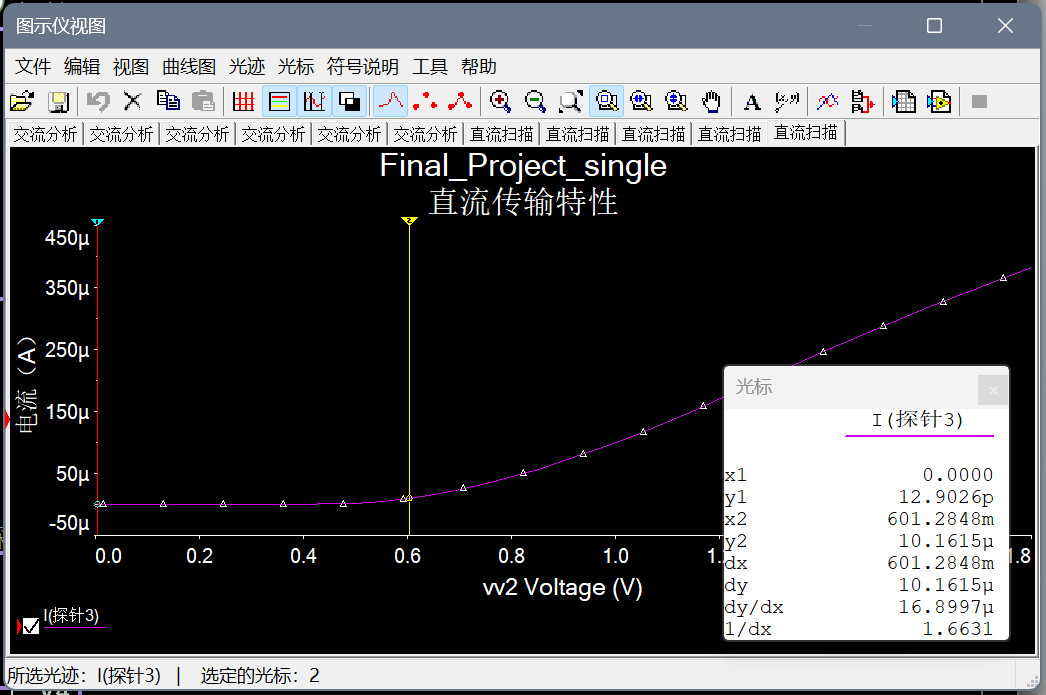
\includegraphics[width=0.35\textwidth]{PMOS_1_12_0.6V_10uA.png}}
\caption{I-V curve of PMOS with W/L=12 }
\label{fig}
\end{figure}

Then, we build the circuit in MULTISIM.

\begin{figure}[htbp]
\centerline{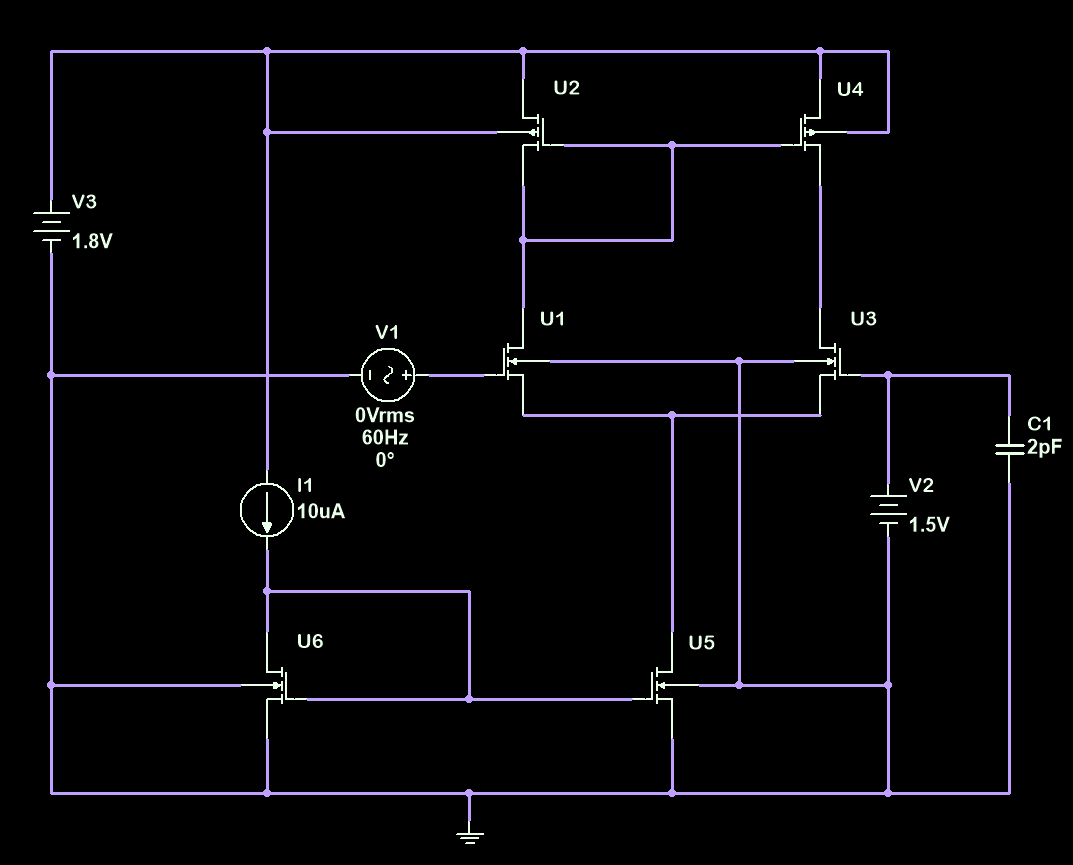
\includegraphics[width=0.35\textwidth]{5 tran pic.png}}
\caption{The circuit of 5 transistor OTA }
\label{fig}
\end{figure}

In this circuit, the NMOS current mirror has transistor widths where one side has a $W/L$ of 3 and the other has a $W/L$ of 6. This configuration mirrors the $10\ \mathrm{\mu A}$ reference current and delivers a $20\ \mathrm{\mu A}$ bias current to the PMOS differential pair.

A common-mode voltage of $0.9\ \mathrm{V}$, along with a very small AC signal as the differential input, is applied to the gates of the differential pair. All MOSFETs in the PMOS current mirror and the differential pair are biased with an absolute gate-source voltage ($V_{GS}$ for NMOS, $V_{SG}$ for PMOS) of $0.6\ \mathrm{V}$ and an absolute drain-source voltage ($|V_{DS}|$) of $0.6\ \mathrm{V}$, ensuring that all transistors operate in the saturation region.


\begin{figure}[htbp]
\centerline{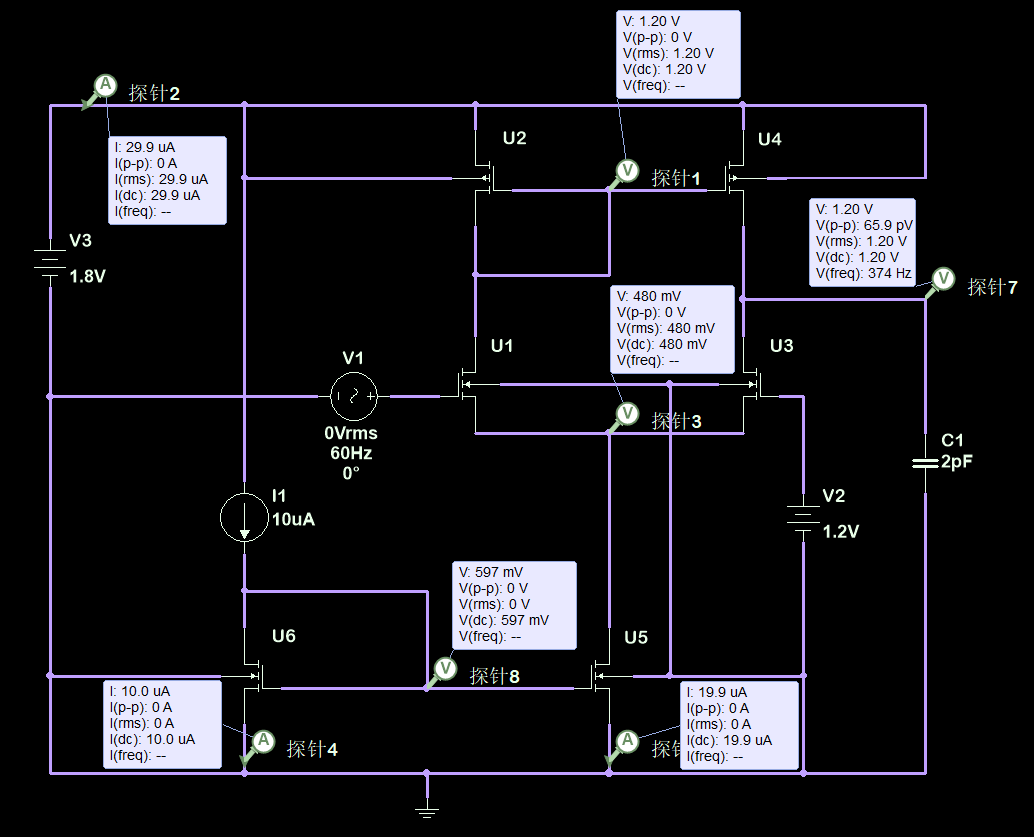
\includegraphics[width=0.35\textwidth]{Open_Loop.png}}
\caption{Node Voltages and Branch Currents in Open-Loop Circuit}
\label{fig}
\end{figure}

\begin{figure}[htbp]
\centerline{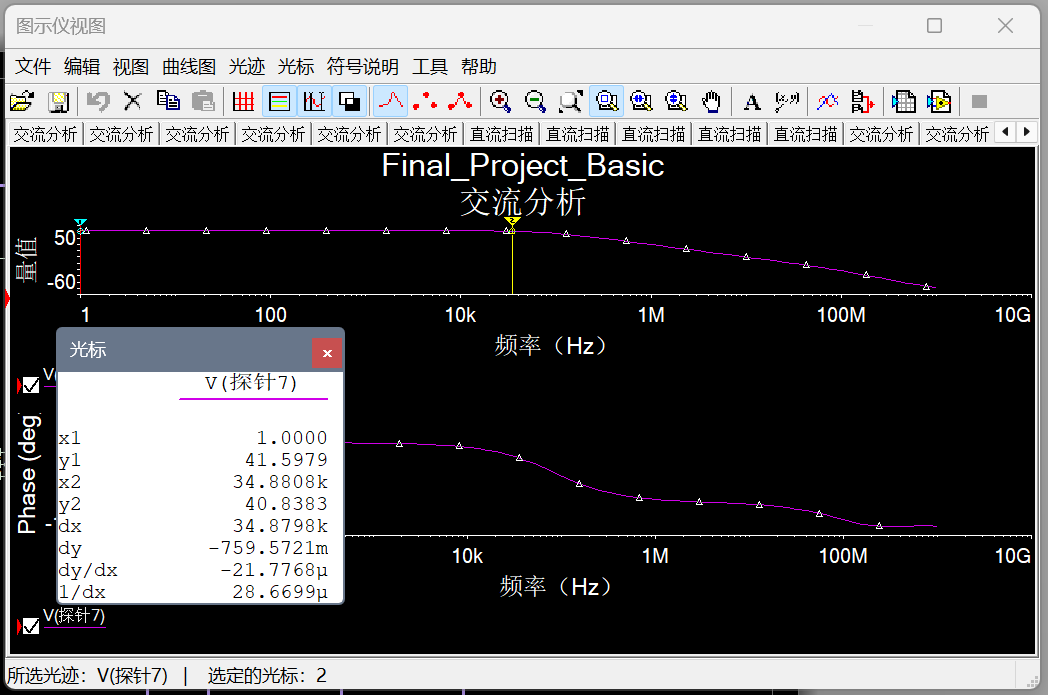
\includegraphics[width=0.35\textwidth]{A_41.5_f_34.88k.png}}
\caption{Simulated AC frequency response of the 5-transistor OTA demonstrating open-loop gain and phase margin}
\label{fig}
\end{figure}

\begin{figure}[htbp]
\centerline{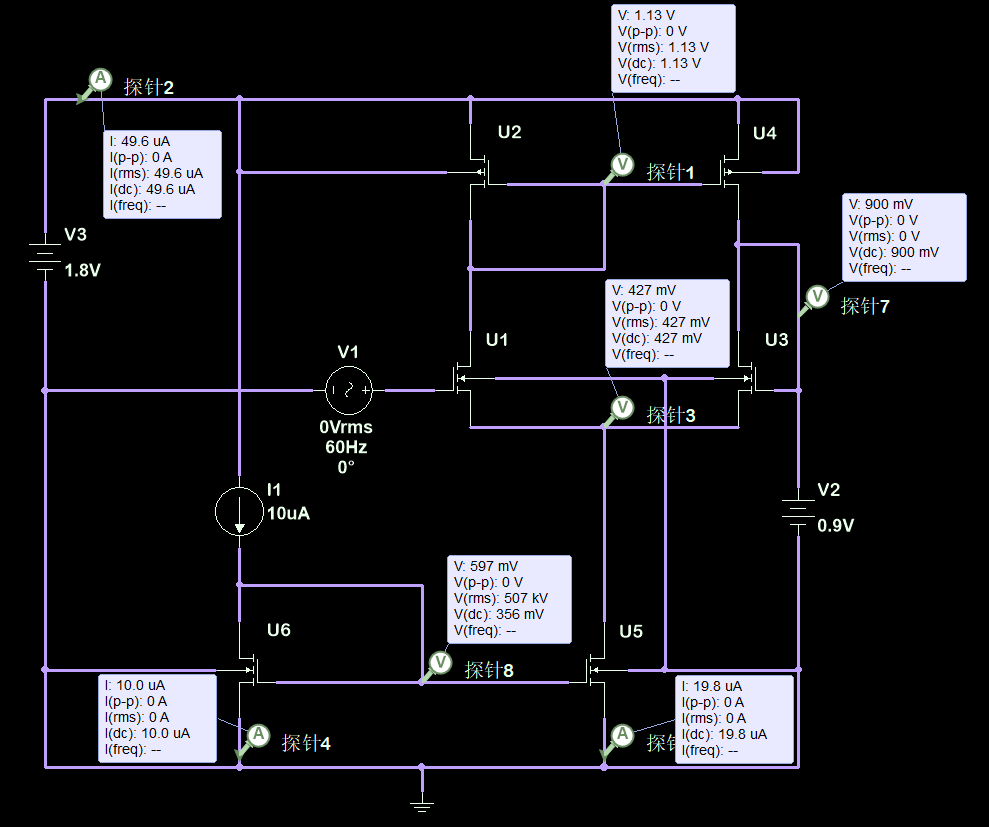
\includegraphics[width=0.35\textwidth]{0.9V_close_loop.png}}
\caption{Node Voltages and Branch Currents in Close-Loop Circuit with 0.9V input}
\label{fig}
\end{figure}

\begin{figure}[htbp]
\centerline{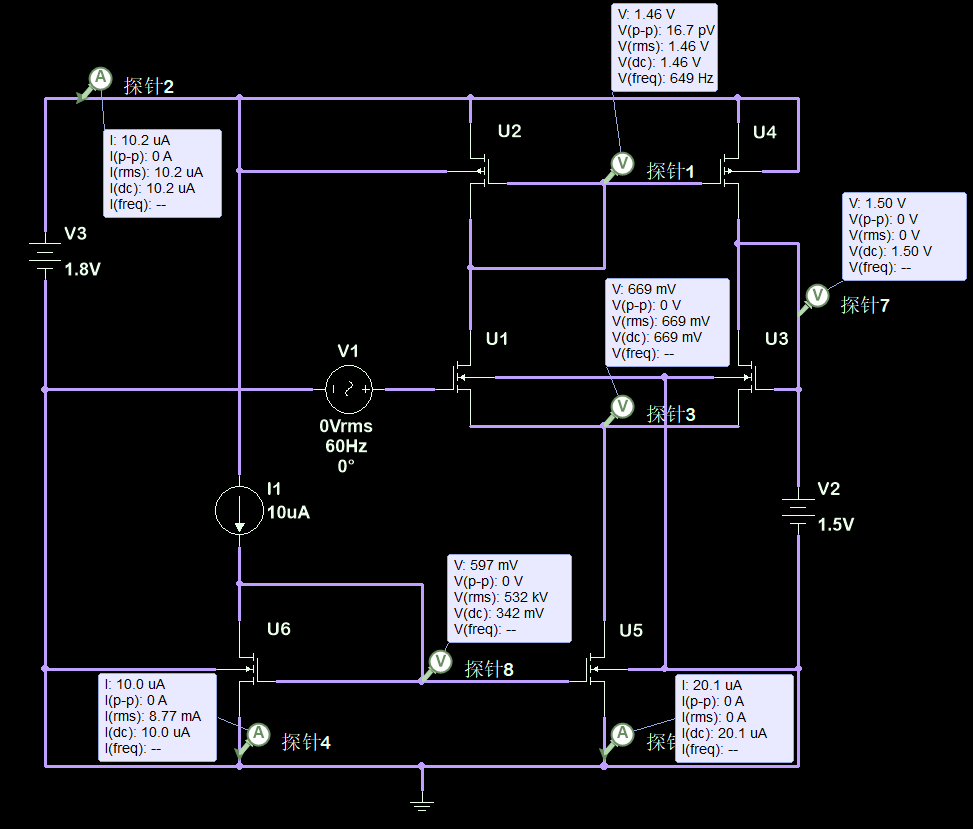
\includegraphics[width=0.35\textwidth]{1.5V_close_loop.png}}
\caption{Node Voltages and Branch Currents in Close-Loop Circuit with 1.5V input}
\label{fig}
\end{figure}

The simulation results demonstrate that the circuit achieves an overall gain of \SI{41.5}{\deci\bel}, with a dominant pole at \SI{34.88}{\kilo\hertz} and a unity-gain frequency of \SI{9.7}{\mega\hertz}. The obtained bandwidth (greater than \SI{30}{\kilo\hertz}) and gain (greater than \SI{40}{\deci\bel}) successfully meet the target specifications.

An examination of the node voltages and branch currents confirms that all MOSFETs are operating in the saturation region, as required for proper amplifier function. Furthermore, the circuit exhibits a reasonable input voltage swing range from \SI{0.9}{\volt} to \SI{1.5}{\volt}, indicating a robust design against variations in the input common-mode level.

\section{3 BIT DAC}
\subsection{Principle}
A DAC transforms a discrete digital code into a precise analog voltage or current. The ideal conversion for an N-bit DAC is governed by the following relationship between the output voltage \( V_{\text{out}} \), the reference voltage \( V_{\text{ref}} \), and the binary input word \( B_{\text{in}} \):

\[
V_{\text{out}} = V_{\text{ref}} \times B_{\text{in}} = V_{\text{ref}} \left( b_1 2^{-1} + b_2 2^{-2} + \cdots + b_N 2^{-N} \right)
\]

where \( b_1 \) is the Most Significant Bit (MSB) and \( b_N \) is the Least Significant Bit (LSB). The fundamental unit of resolution, the voltage corresponding to 1 LSB, is defined as:

\[
V_{\text{LSB}} = \frac{V_{\text{ref}}}{2^N}
\]

\subsubsection{Resistor-Based Implementation (R-2R Ladder)}

A common physical realization uses an R-2R ladder network. The key to its operation is that the equivalent resistance looking into any node is \( 2R \), creating binary-weighted currents.[1] The current for the \( i \)-th branch is:

\[
I_i = \frac{V_{\text{ref}}}{2R} \cdot \frac{1}{2^{i-1}} = \frac{V_{\text{ref}}}{2^i R}
\]

The total output current for a given digital input is the sum of the currents of the active (\( b_i = 1 \)) branches:

\[
I_{\text{out}} = \sum_{i=1}^{N} b_i \cdot I_i = \frac{V_{\text{ref}}}{R} \sum_{i=1}^{N} \frac{b_i}{2^i}
\]

This current is typically converted to a voltage using an operational amplifier with feedback resistor \( R_F \):

\[
V_{\text{out}} = - R_F \cdot I_{\text{out}} = - V_{\text{ref}} \frac{R_F}{R} \sum_{i=1}^{N} \frac{b_i}{2^i}
\]

\subsubsection{Performance Metrics: Linearity Error}

The precision of a DAC is quantified by its linearity errors, which stem from component mismatches (e.g., resistors).

\begin{itemize}
    \item \textbf{Differential Nonlinearity (DNL)} is the deviation of the actual step size from the ideal 1 LSB value:

    \[
    \text{DNL}_i = \frac{V_{\text{out}}(i) - V_{\text{out}}(i-1)}{V_{\text{LSB}}} - 1
    \]
    where \( V_{\text{out}}(i) \) is the output voltage for digital code \( i \).

    \item \textbf{Integral Nonlinearity (INL)} is the cumulative deviation of the actual transfer curve from a best-fit straight line after removing offset and gain errors:

    \[
    \text{INL}_i = \frac{V_{\text{out}}(i) - V_{\text{ideal}}(i)}{V_{\text{LSB}}}
    \]
\end{itemize}

\begin{figure}[htbp]
\centerline{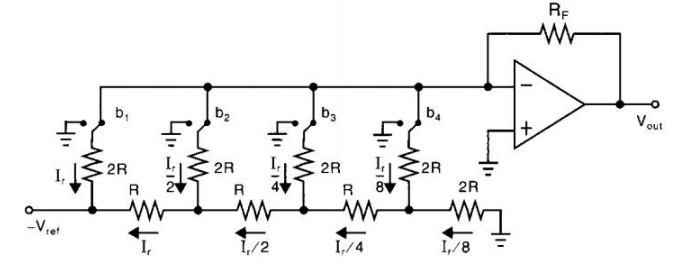
\includegraphics[width=0.35\textwidth]{Diagram of DAC.png}}
\caption{Diagram of 4-bit DAC circuit}
\label{fig}
\end{figure}

\subsection{The structure}

\begin{figure}[htbp]
\centerline{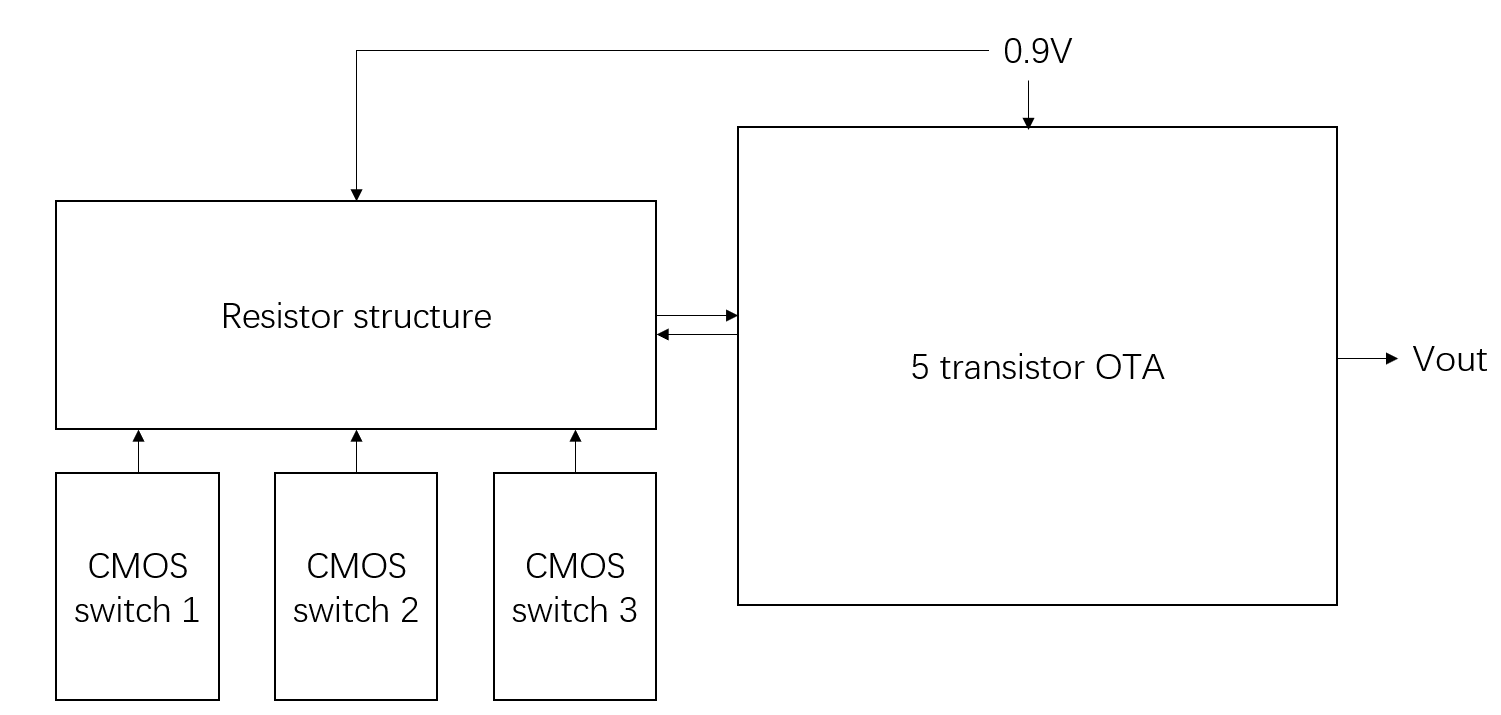
\includegraphics[width=0.35\textwidth]{structure of DAC.png}}
\caption{Schematic of the 3-bit DAC topology}
\label{fig}
\end{figure}

A 3-bit DAC consists of three parts. The first part is the input stage. The complementary transmission gate switch is composed of two NMOS transistors connected in parallel. The gates of these two transistors are driven by a pair of complementary control signals. This complementary structure, by connecting the transistors in parallel, provides a smaller and more stable resistance when path is ON, ensuring consistency in the current path impedance across different input codes.

If a 1.8V high-level signal is applied, the gate of one NMOS is pulled up to 1.8V, and the entire path is considered ON, meaning the input is `1'. If a low-level signal is applied, both MOS transistors will turn OFF, blocking current flow. The second part is the R-2R Ladder Resistor Network. Through current splitting and parallel flow via resistors, the current I is divided into I/2, I/4, and I/8 to achieve per-bit control. The output is then fed into a 5-transistor OTA. The 5-transistor OTA acts as an operational amplifier, amplifying the signal and providing the output.


\subsection{Circuit Implementation}
\begin{figure}[htbp]
\centerline{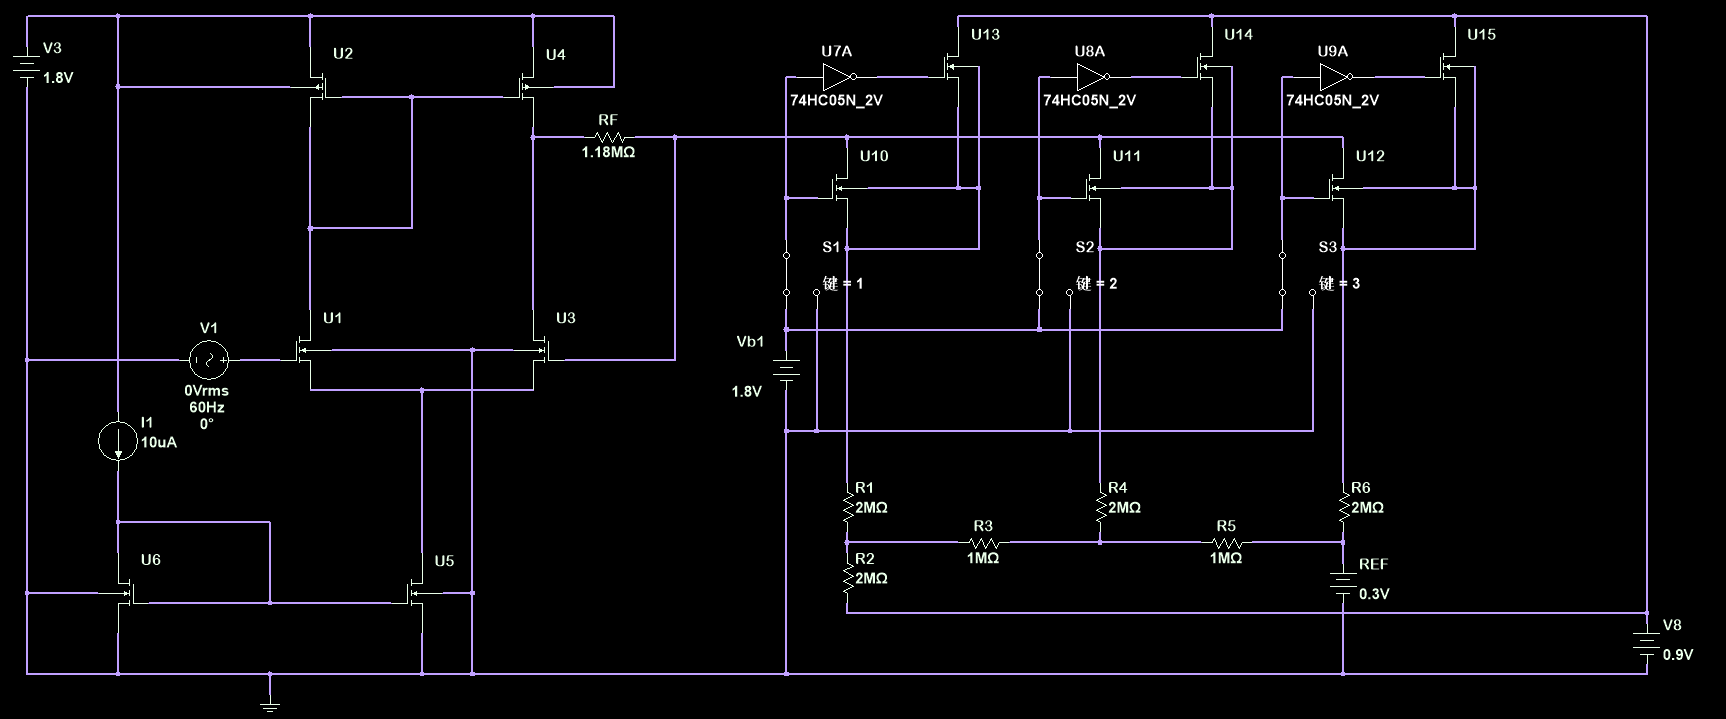
\includegraphics[width=0.48\textwidth]{circuit.png}}
\caption{3-BIT DAC circuit}
\label{fig}
\end{figure}


In the circuit, we select $R = \SI{1}{\mega\ohm}$ to raise the resistance, thereby minimizing the impact of switch operation on the current. The feedback resistor is set to $R_f = \SI{1.03}{\mega\ohm}$. This value ensures that the maximum output voltage is \SI{1.425}{\volt}, matching the theoretical value and thus reducing error. Furthermore, the $W/L$ ratio of each MOS transistor is set to 100 to achieve a smaller path resistance. The parameters of the 5-transistor OTA remain unchanged.

Since the differential pair requires a \SI{0.9}{\volt} common-mode voltage as an additional input, the ground level of the resistor network is raised to \SI{0.9}{\volt} to balance the overall DC operating point. Consequently, the entire core circuit uses \SI{0.9}{\volt} as its ground reference. The reference voltage is set as $V_{\text{ref}} = \text{LSB} \times 8 = \SI{0.3}{\volt}$. Within the circuit, $-V_{\text{ref}}$ is then level-shifted by \SI{0.9}{\volt}, resulting in a final voltage of \SI{0.6}{\volt}.


\begin{figure}[htbp]
\centerline{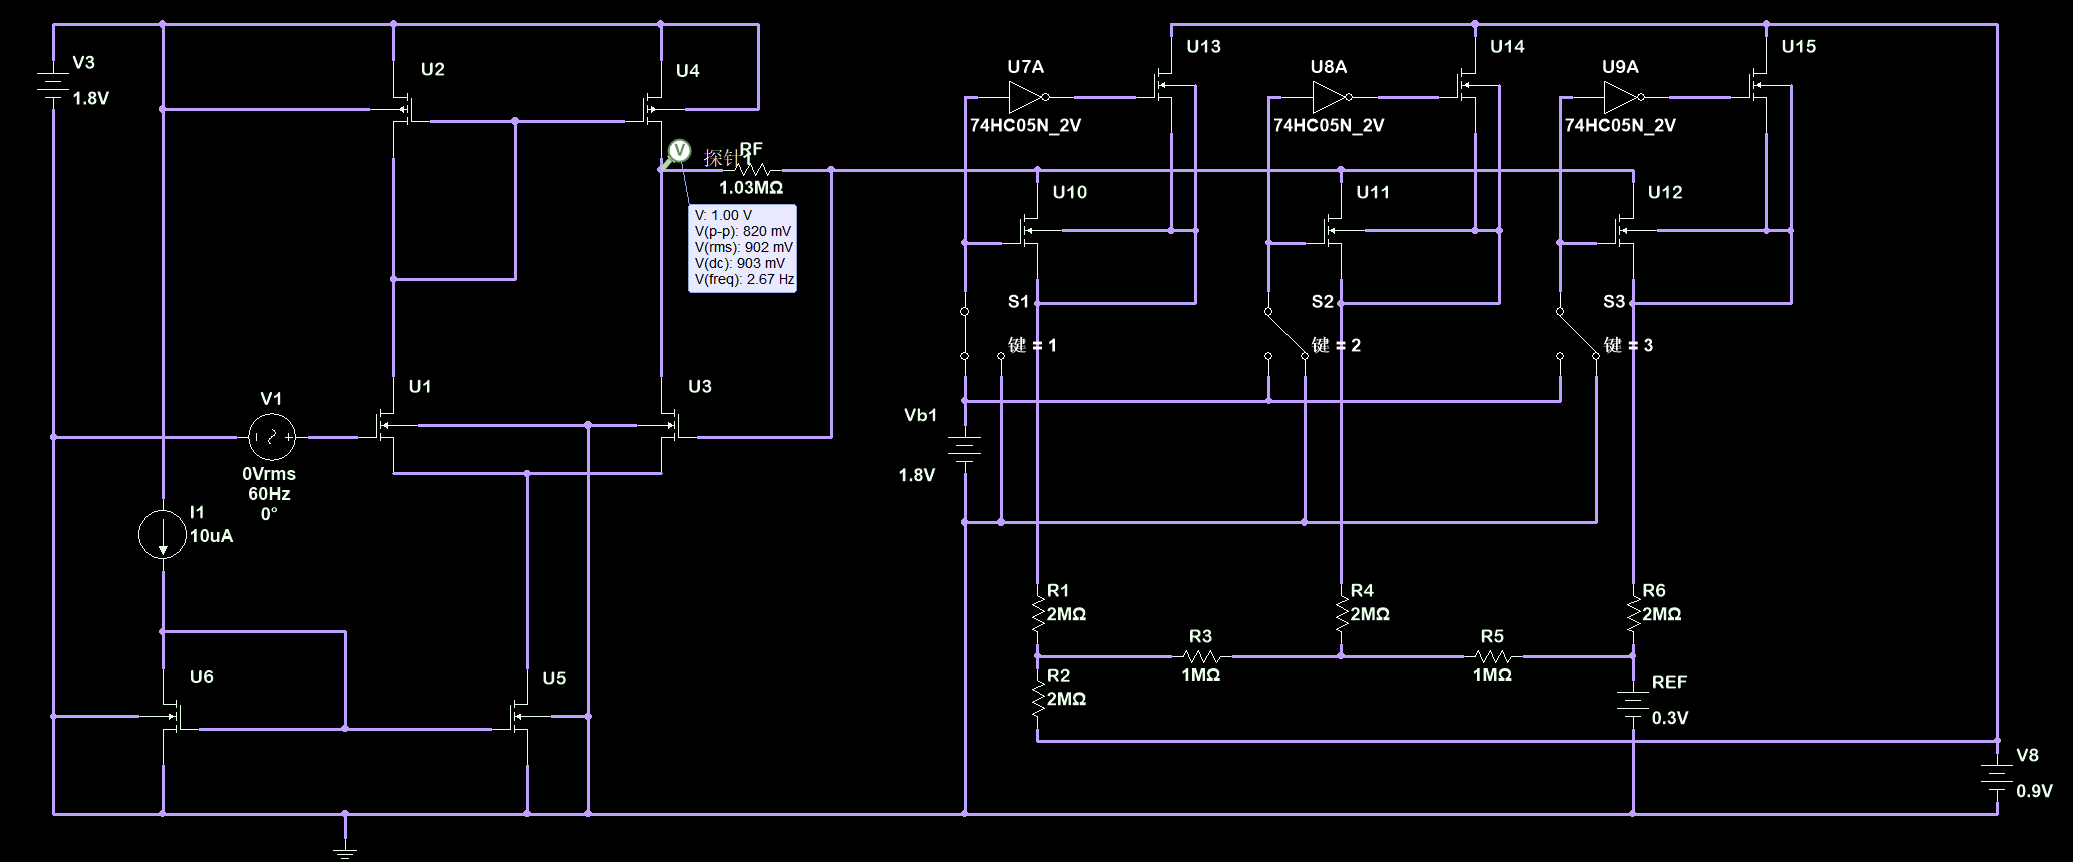
\includegraphics[width=0.48\textwidth]{001_output.png}}
\caption{The output with input 001}
\label{fig}
\end{figure}

\begin{figure}[htbp]
\centerline{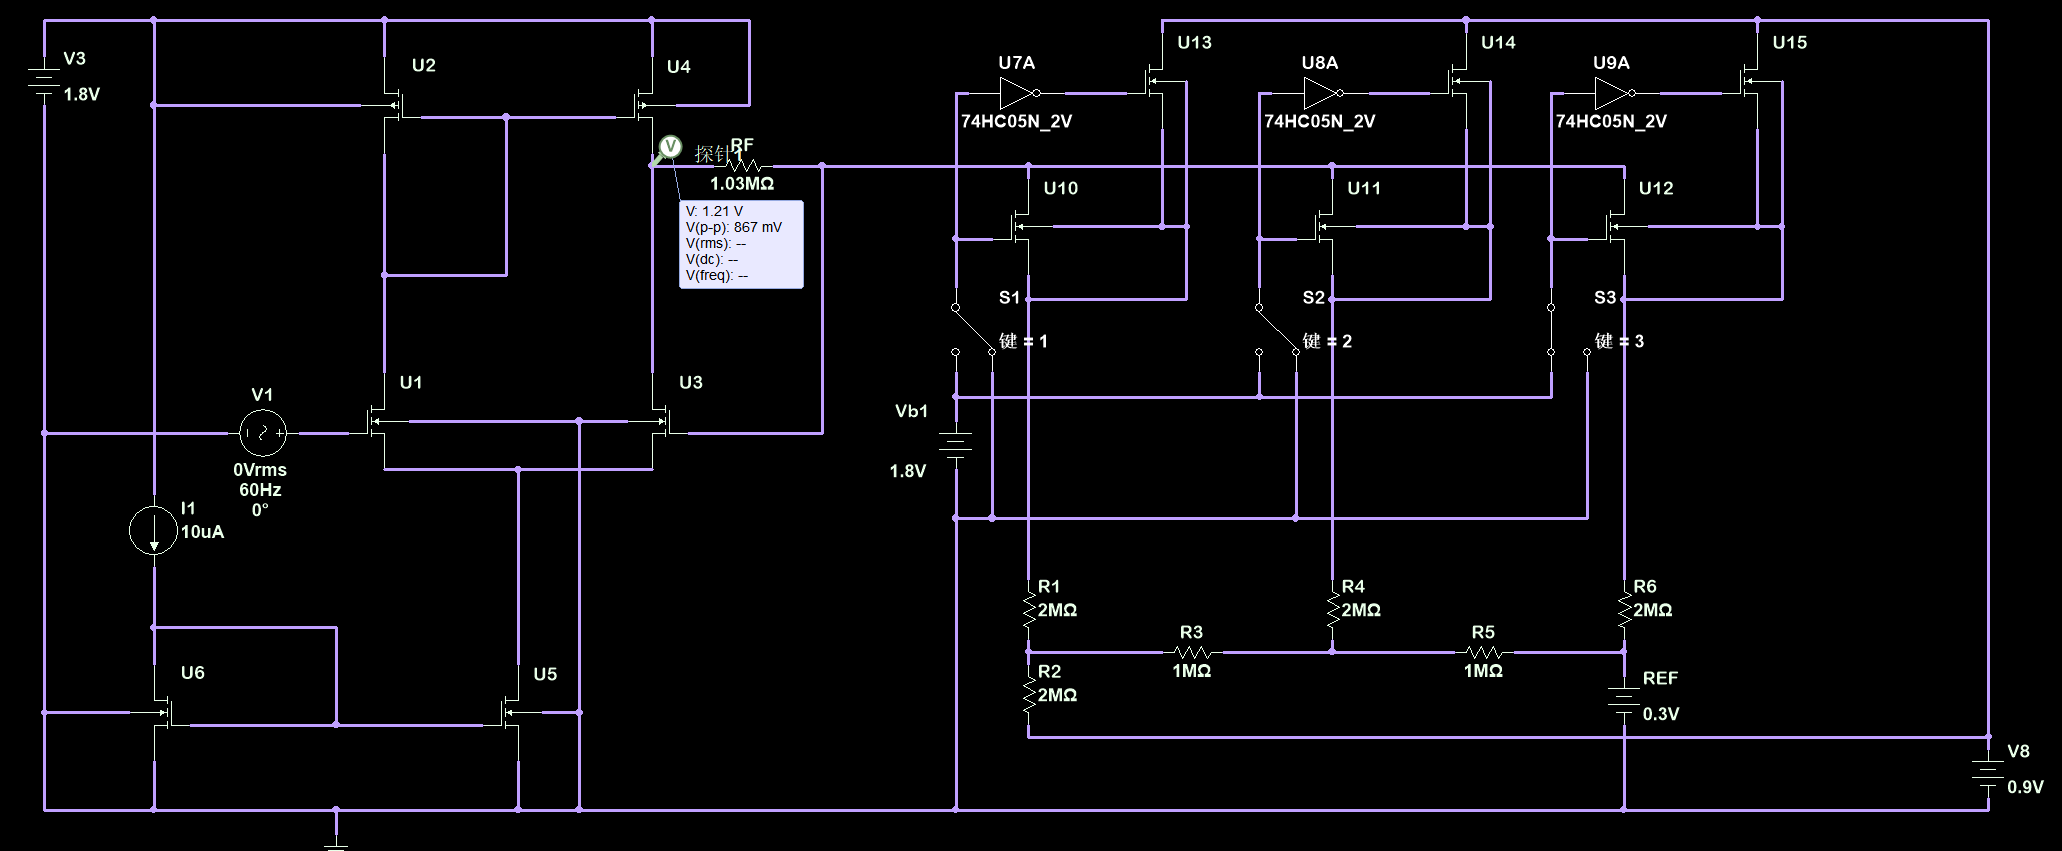
\includegraphics[width=0.48\textwidth]{100_output.png}}
\caption{The output with input 100}
\label{fig}
\end{figure}

\begin{figure}[htbp]
\centerline{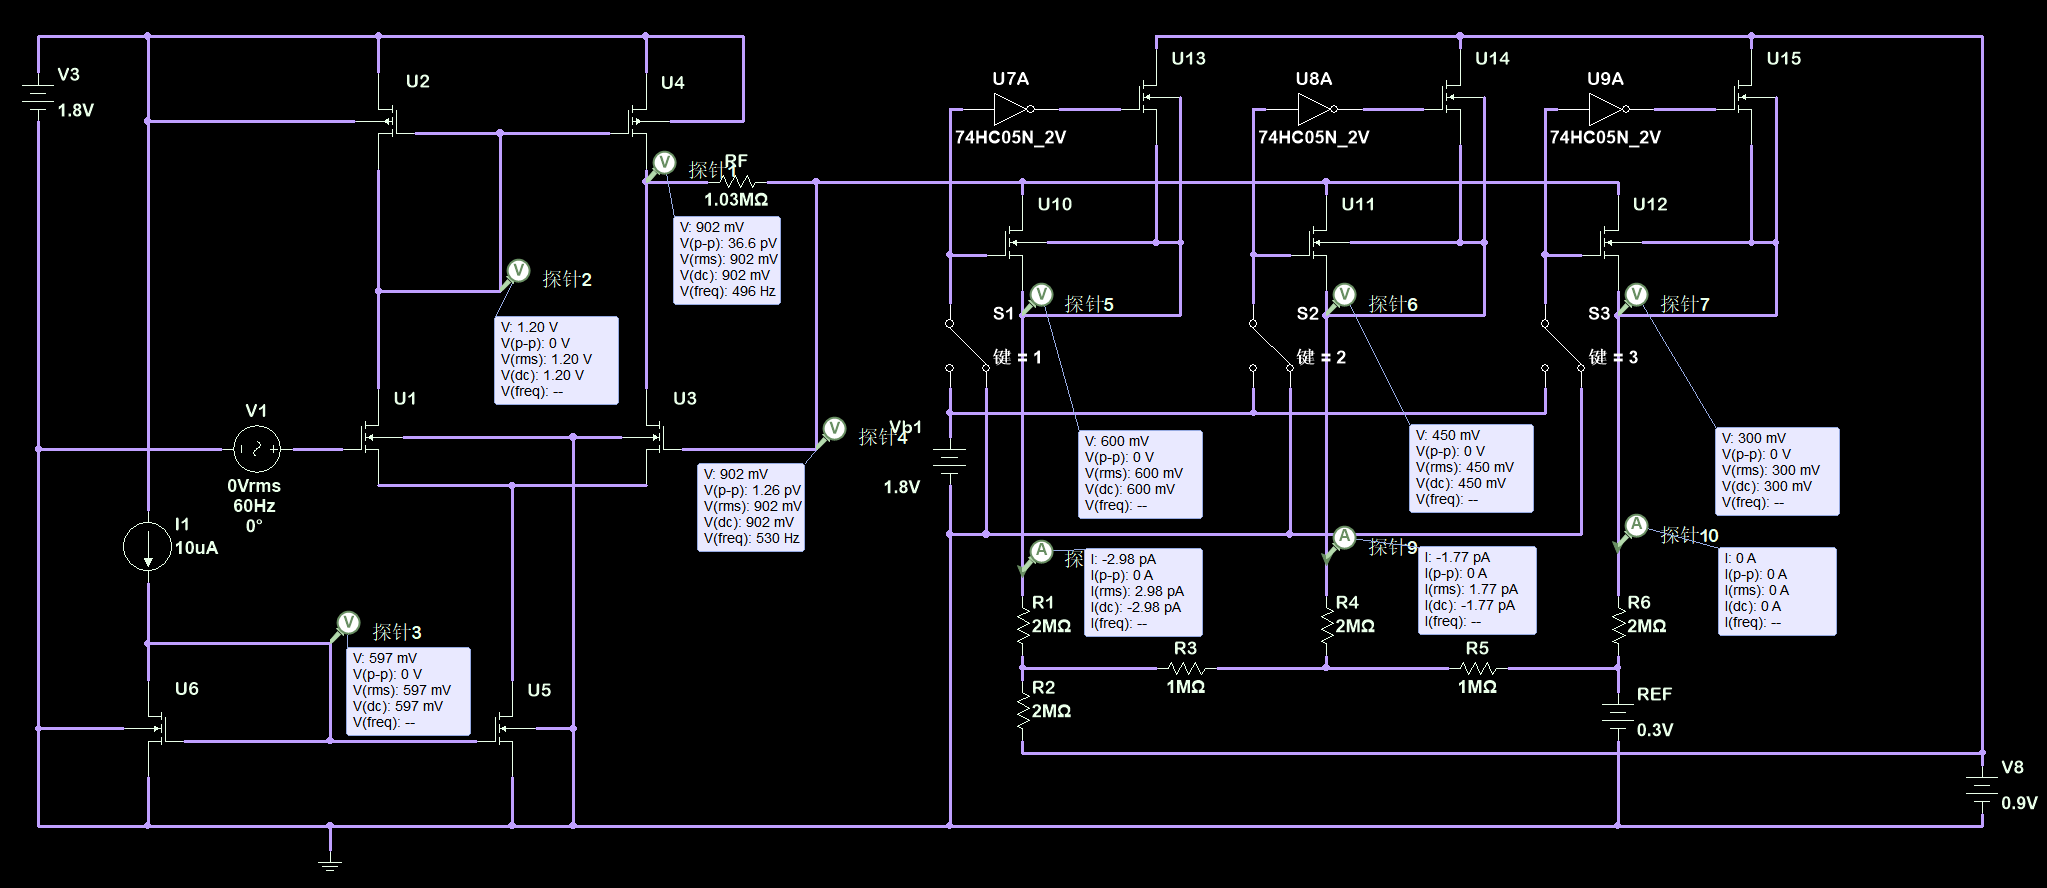
\includegraphics[width=0.48\textwidth]{000.png}}
\caption{Node Voltages and Branch Currents in Close-Loop Circuit with input 000}
\label{fig}
\end{figure}


\begin{figure}[htbp]
\centerline{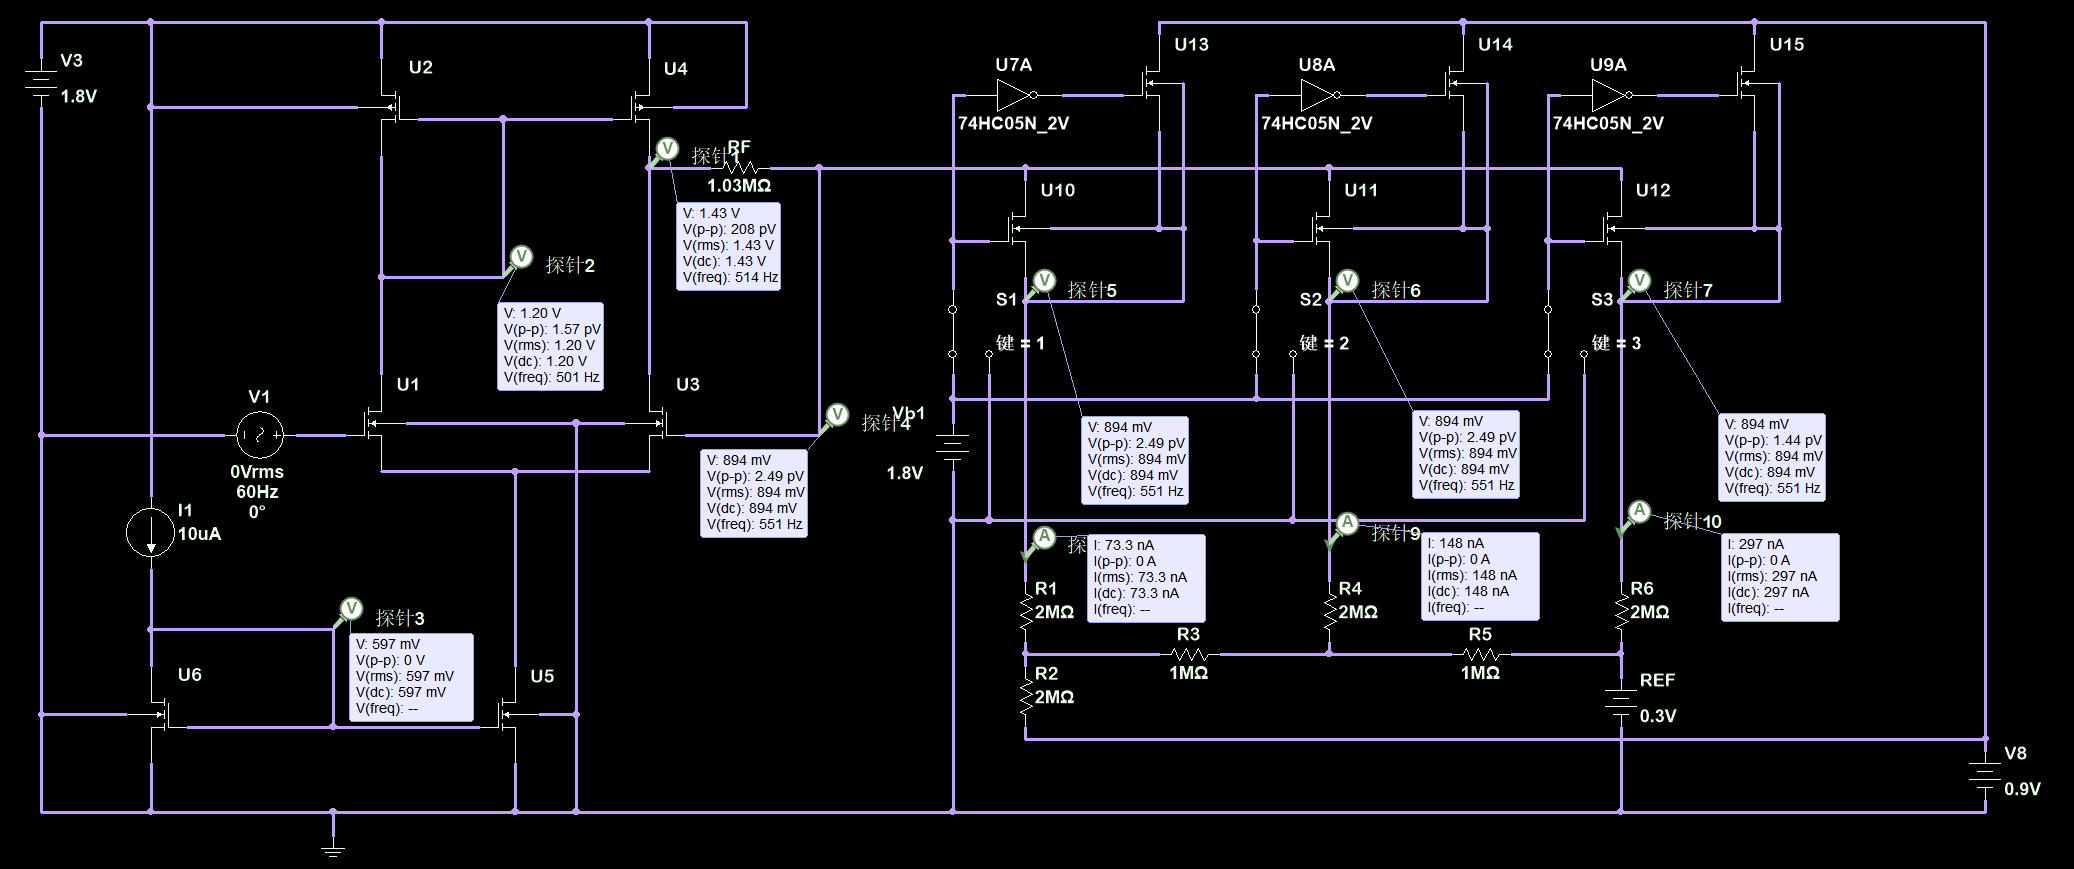
\includegraphics[width=0.48\textwidth]{111.png}}
\caption{Node Voltages and Branch Currents in Close-Loop Circuit with input 111}
\label{fig}
\end{figure}


Based on the node voltages, all MOS transistors are biased in the saturation region, confirming proper circuit operation.

\begin{table}[htbp]
\caption{DNL and INL Measurement Results}
\begin{center}
\begin{tabular}{|c|c|c|c|c|}
\hline
\textbf{Table}&\multicolumn{4}{|c|}{\textbf{Measurement Results}} \\
\cline{2-5} 
\textbf{Input} & \textbf{\textit{$V_{The}$ (V)}}& \textbf{\textit{$V_{Stimu}$ (V)}}& \textbf{\textit{$|DNL| (LSB)$}}& \textbf{\textit{$|INL| (LSB)$}} \\
\hline
000 & 0.900 & 0.902 & - & 0.027 \\
\hline
001 & 0.975 & 1.000 & 0.31 & 0.33 \\
\hline
010 & 1.050 & 1.070 & 0.07 & 0.27 \\
\hline
011 & 1.125 & 1.130 & 0.20 & 0.07 \\
\hline
100 & 1.200 & 1.210 & 0.07 & 0.13 \\
\hline
101 & 1.275 & 1.300 & 0.20 & 0.33 \\
\hline
110 & 1.350 & 1.370 & 0.07 & 0.27 \\
\hline
111 & 1.425 & 1.430 & 0.20 & 0.07 \\
\hline
\end{tabular}
\label{tab1}
\end{center}
\end{table}


The final simulation results indicate that all differential nonlinearity (DNL) and integral nonlinearity (INL) errors are less than \SI{0.5}{LSB} and \SI{1}{LSB}, respectively. This confirms excellent circuit performance from the simulation, guaranteeing no code missing or non-monotonic behavior. The maximum DNL error is only \SI{0.31}{LSB} (at the code transition corresponding to input `001`), and the maximum INL error is \SI{0.33}{LSB} (at the transitions for inputs `001` and `101`).

\begin{figure}[htbp]
\centerline{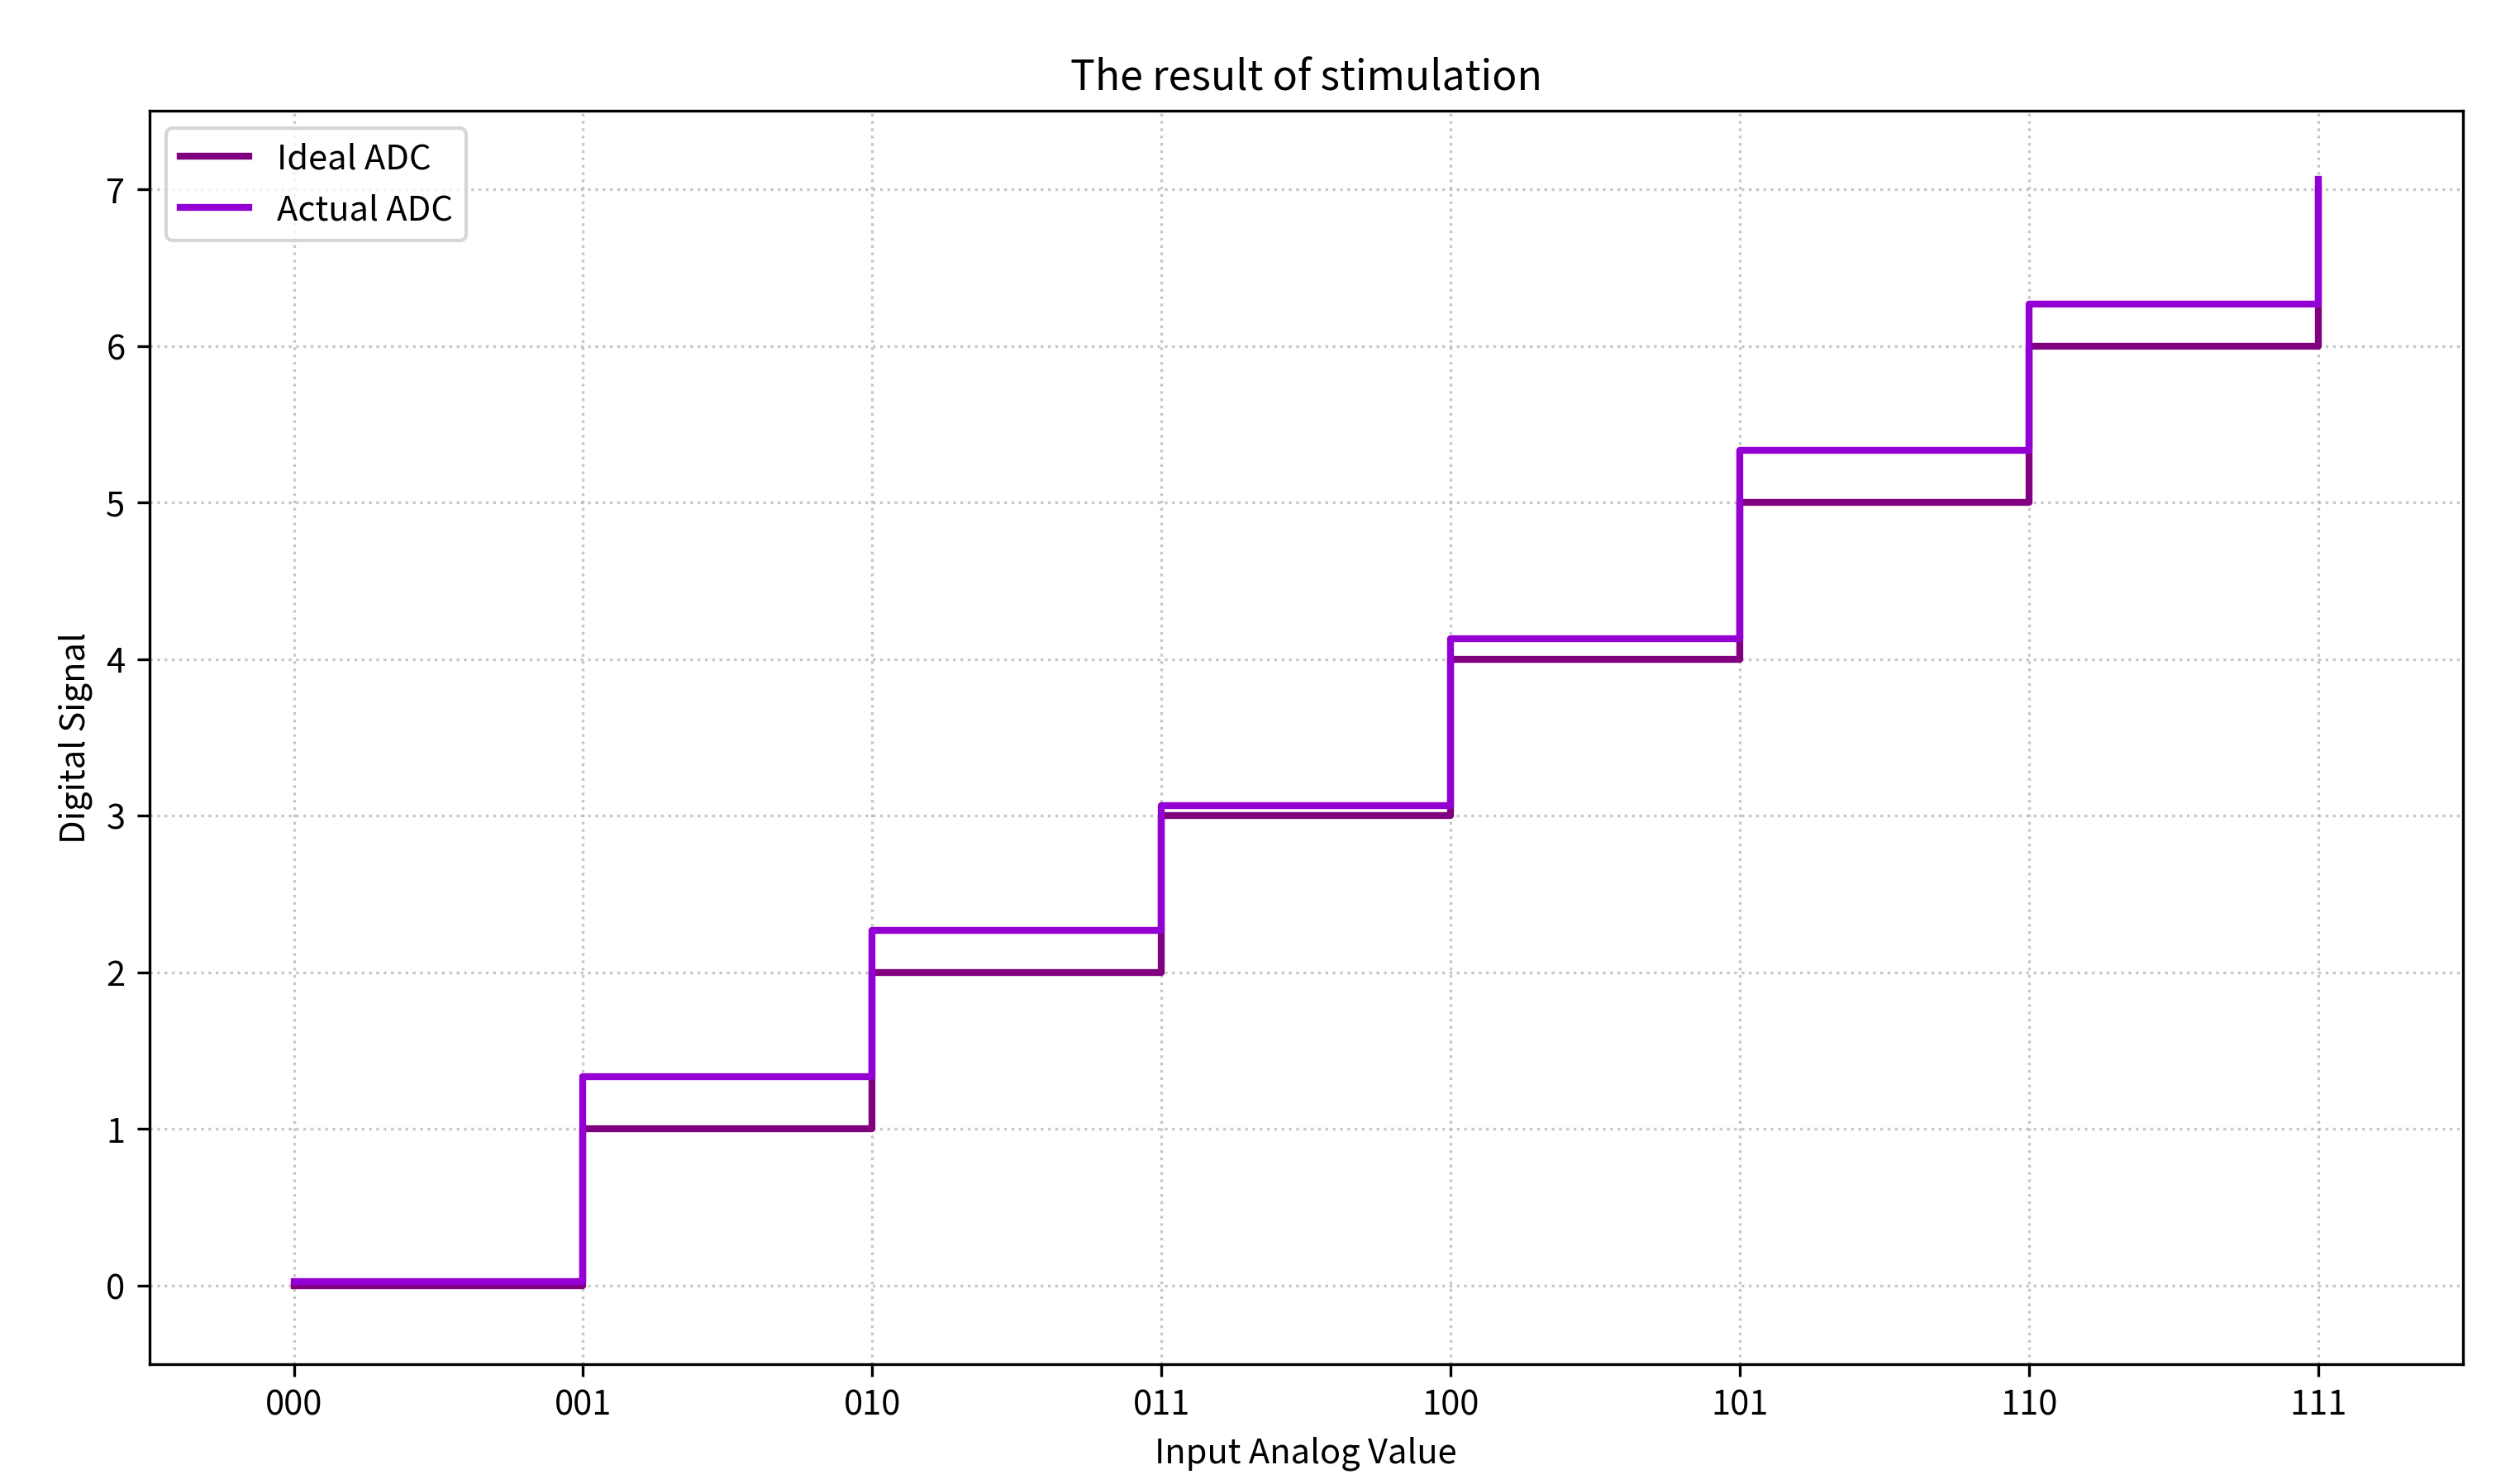
\includegraphics[width=0.48\textwidth]{the result 1.png}}
\caption{The Stepped Chart of $V_{out}$ in theory and under stimulation}
\label{fig}
\end{figure}

\begin{figure}[htbp]
\centerline{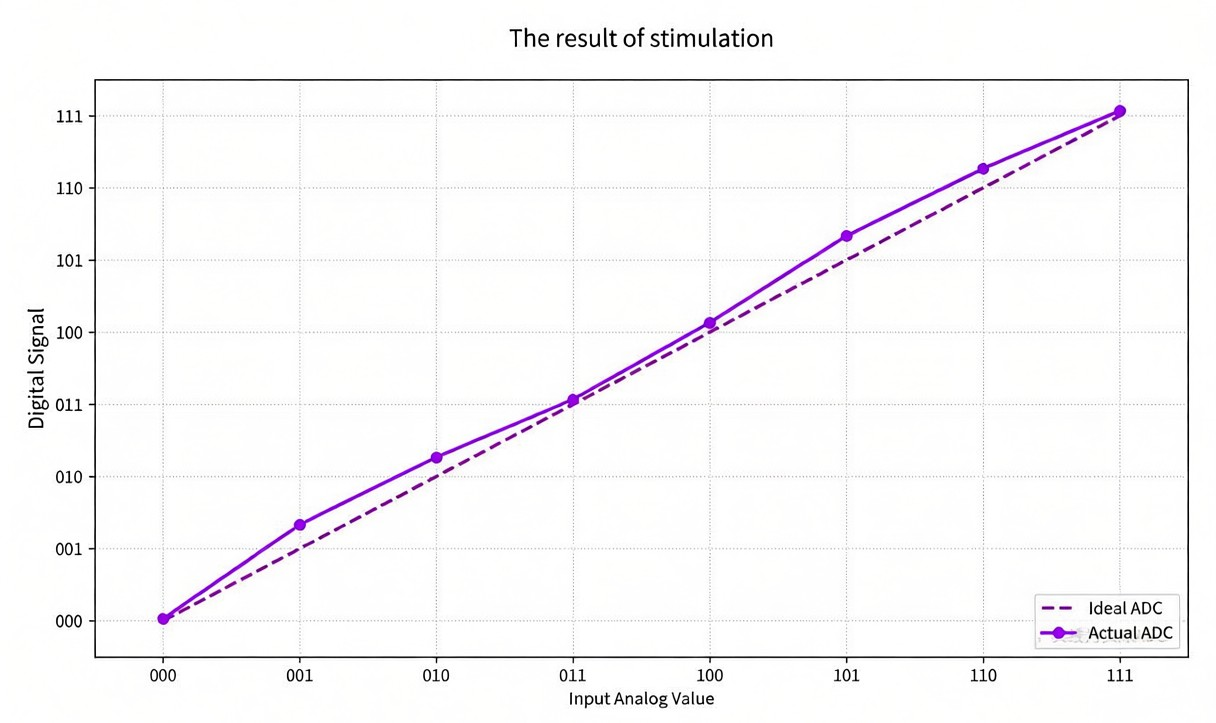
\includegraphics[width=0.48\textwidth]{the result 2.jpeg}}
\caption{The line chart of $V_{out}$ in theory and under stimulation}
\label{fig}
\end{figure}

\begin{figure}[htbp]
\centerline{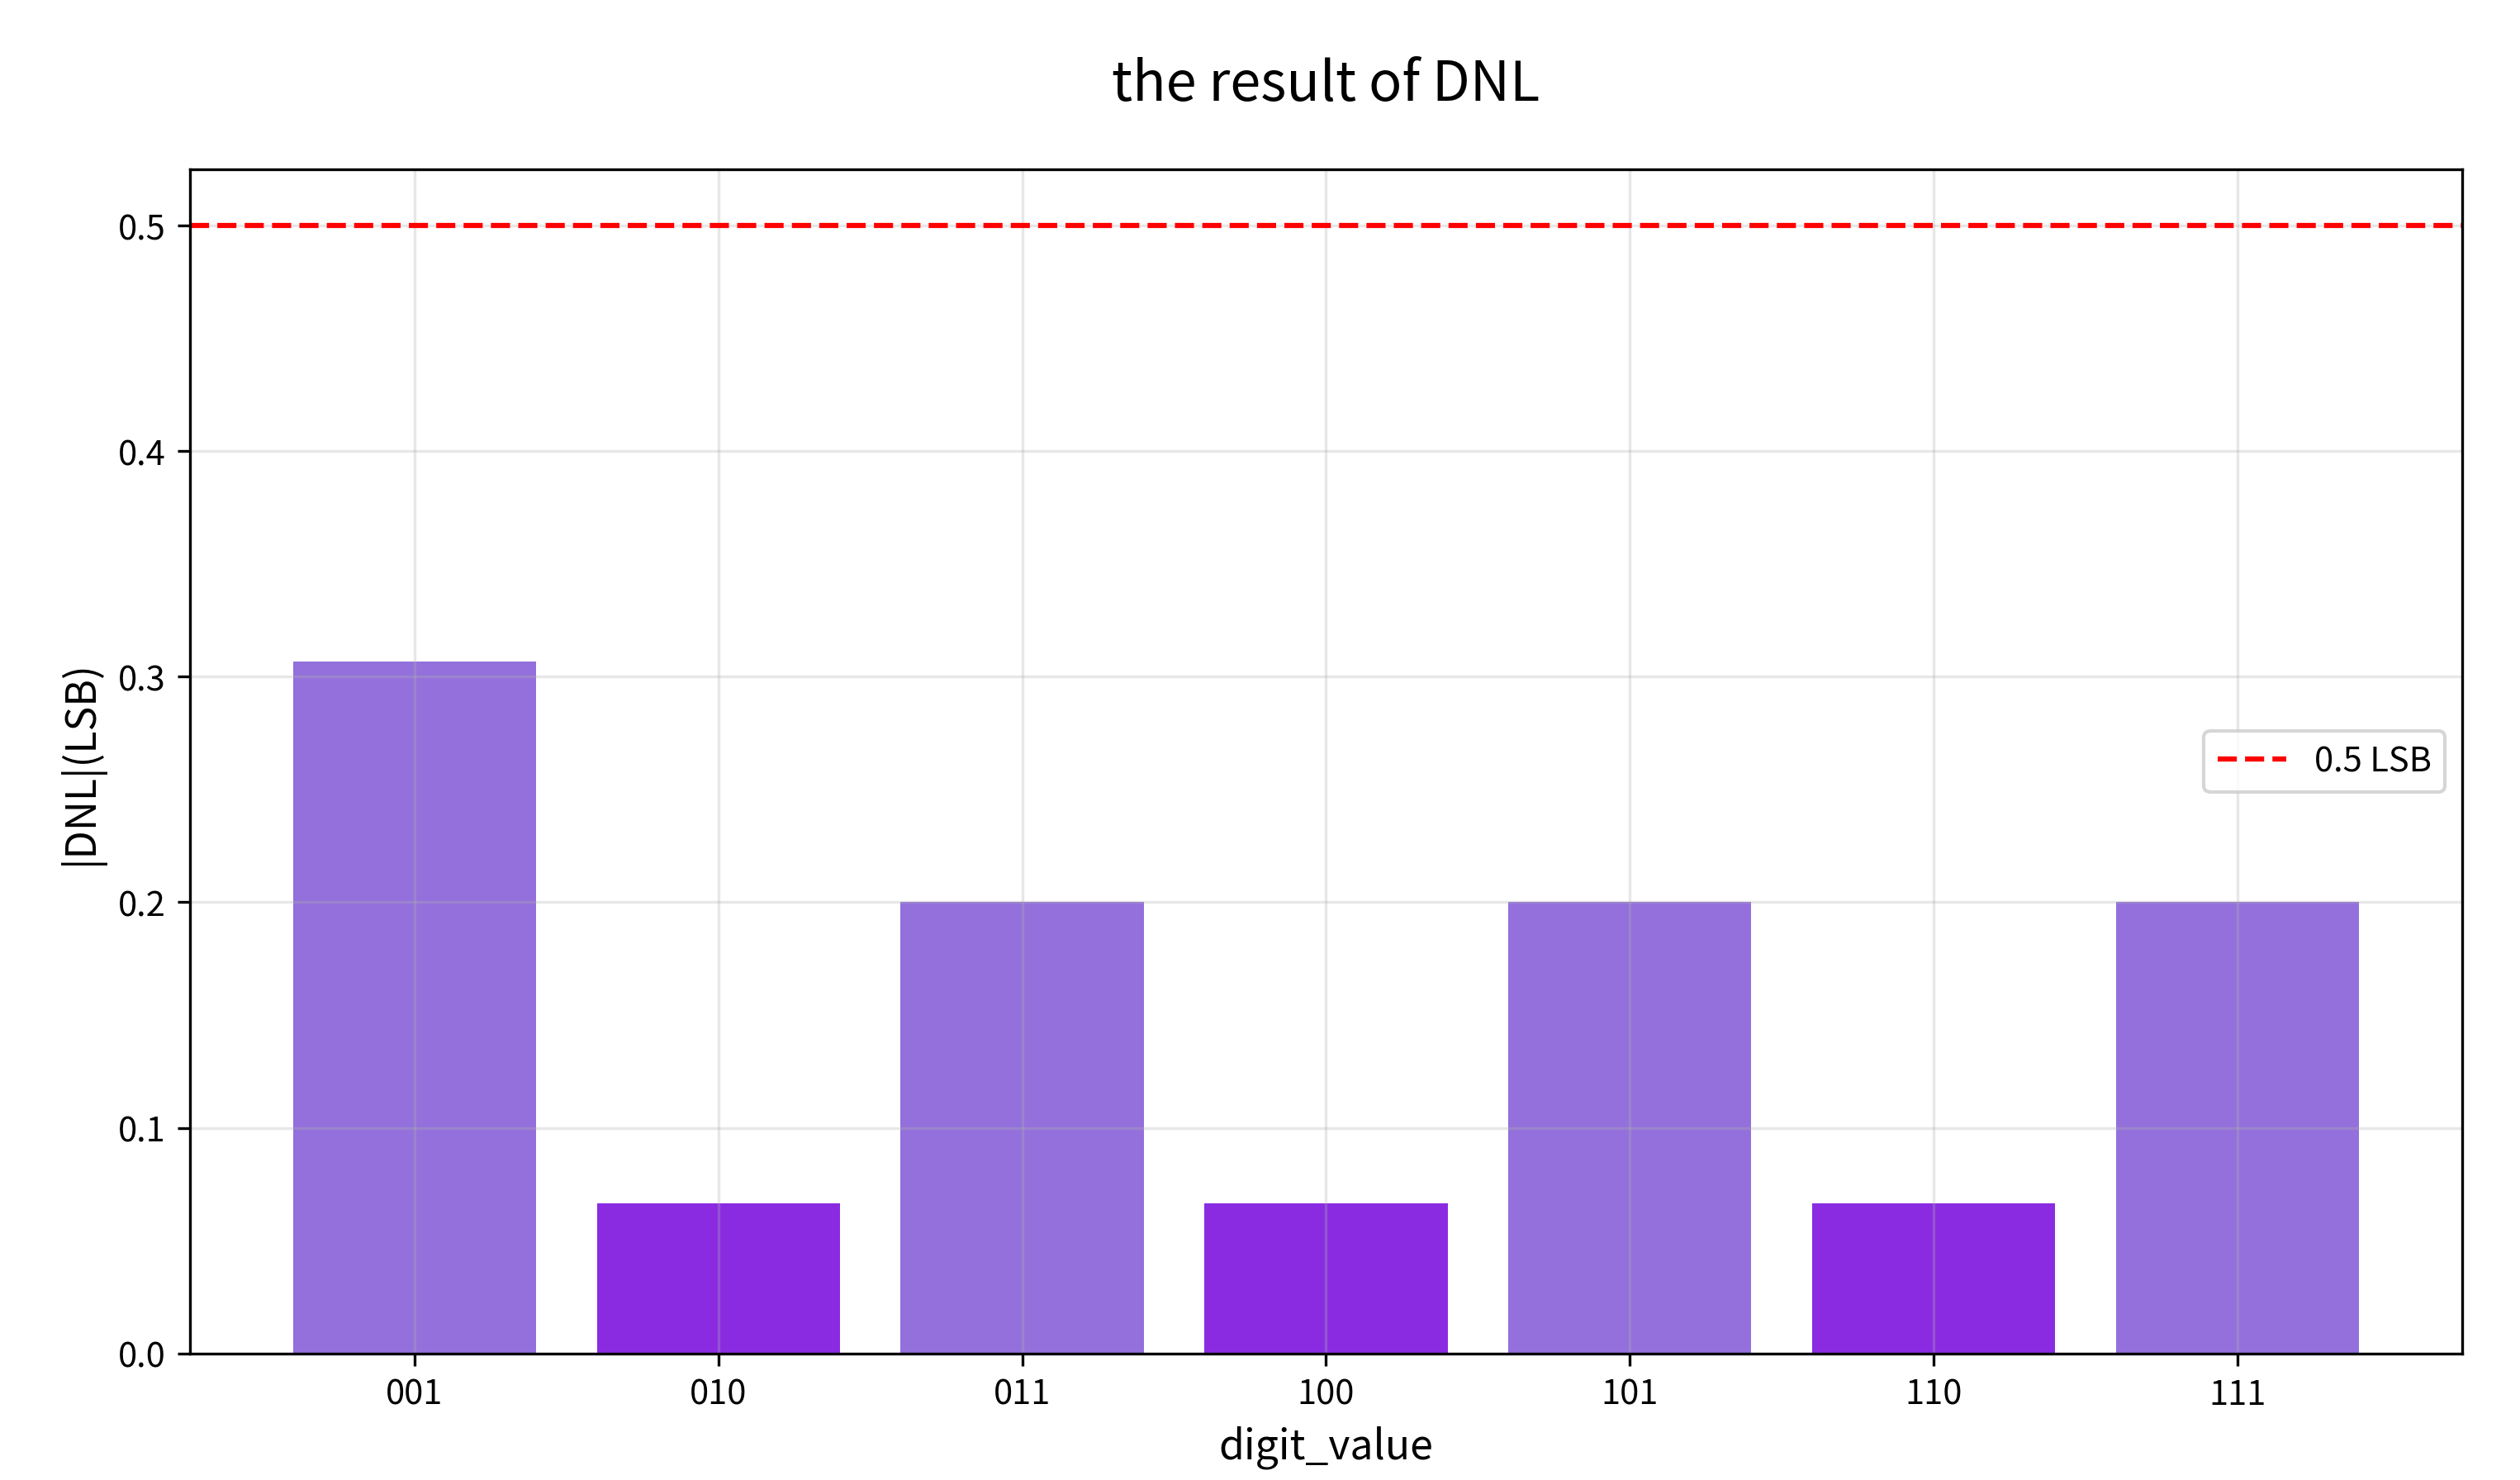
\includegraphics[width=0.48\textwidth]{the result 4 DNL.png}}
\caption{Bar Chart of DNL}
\label{fig}
\end{figure}

\begin{figure}[htbp]
\centerline{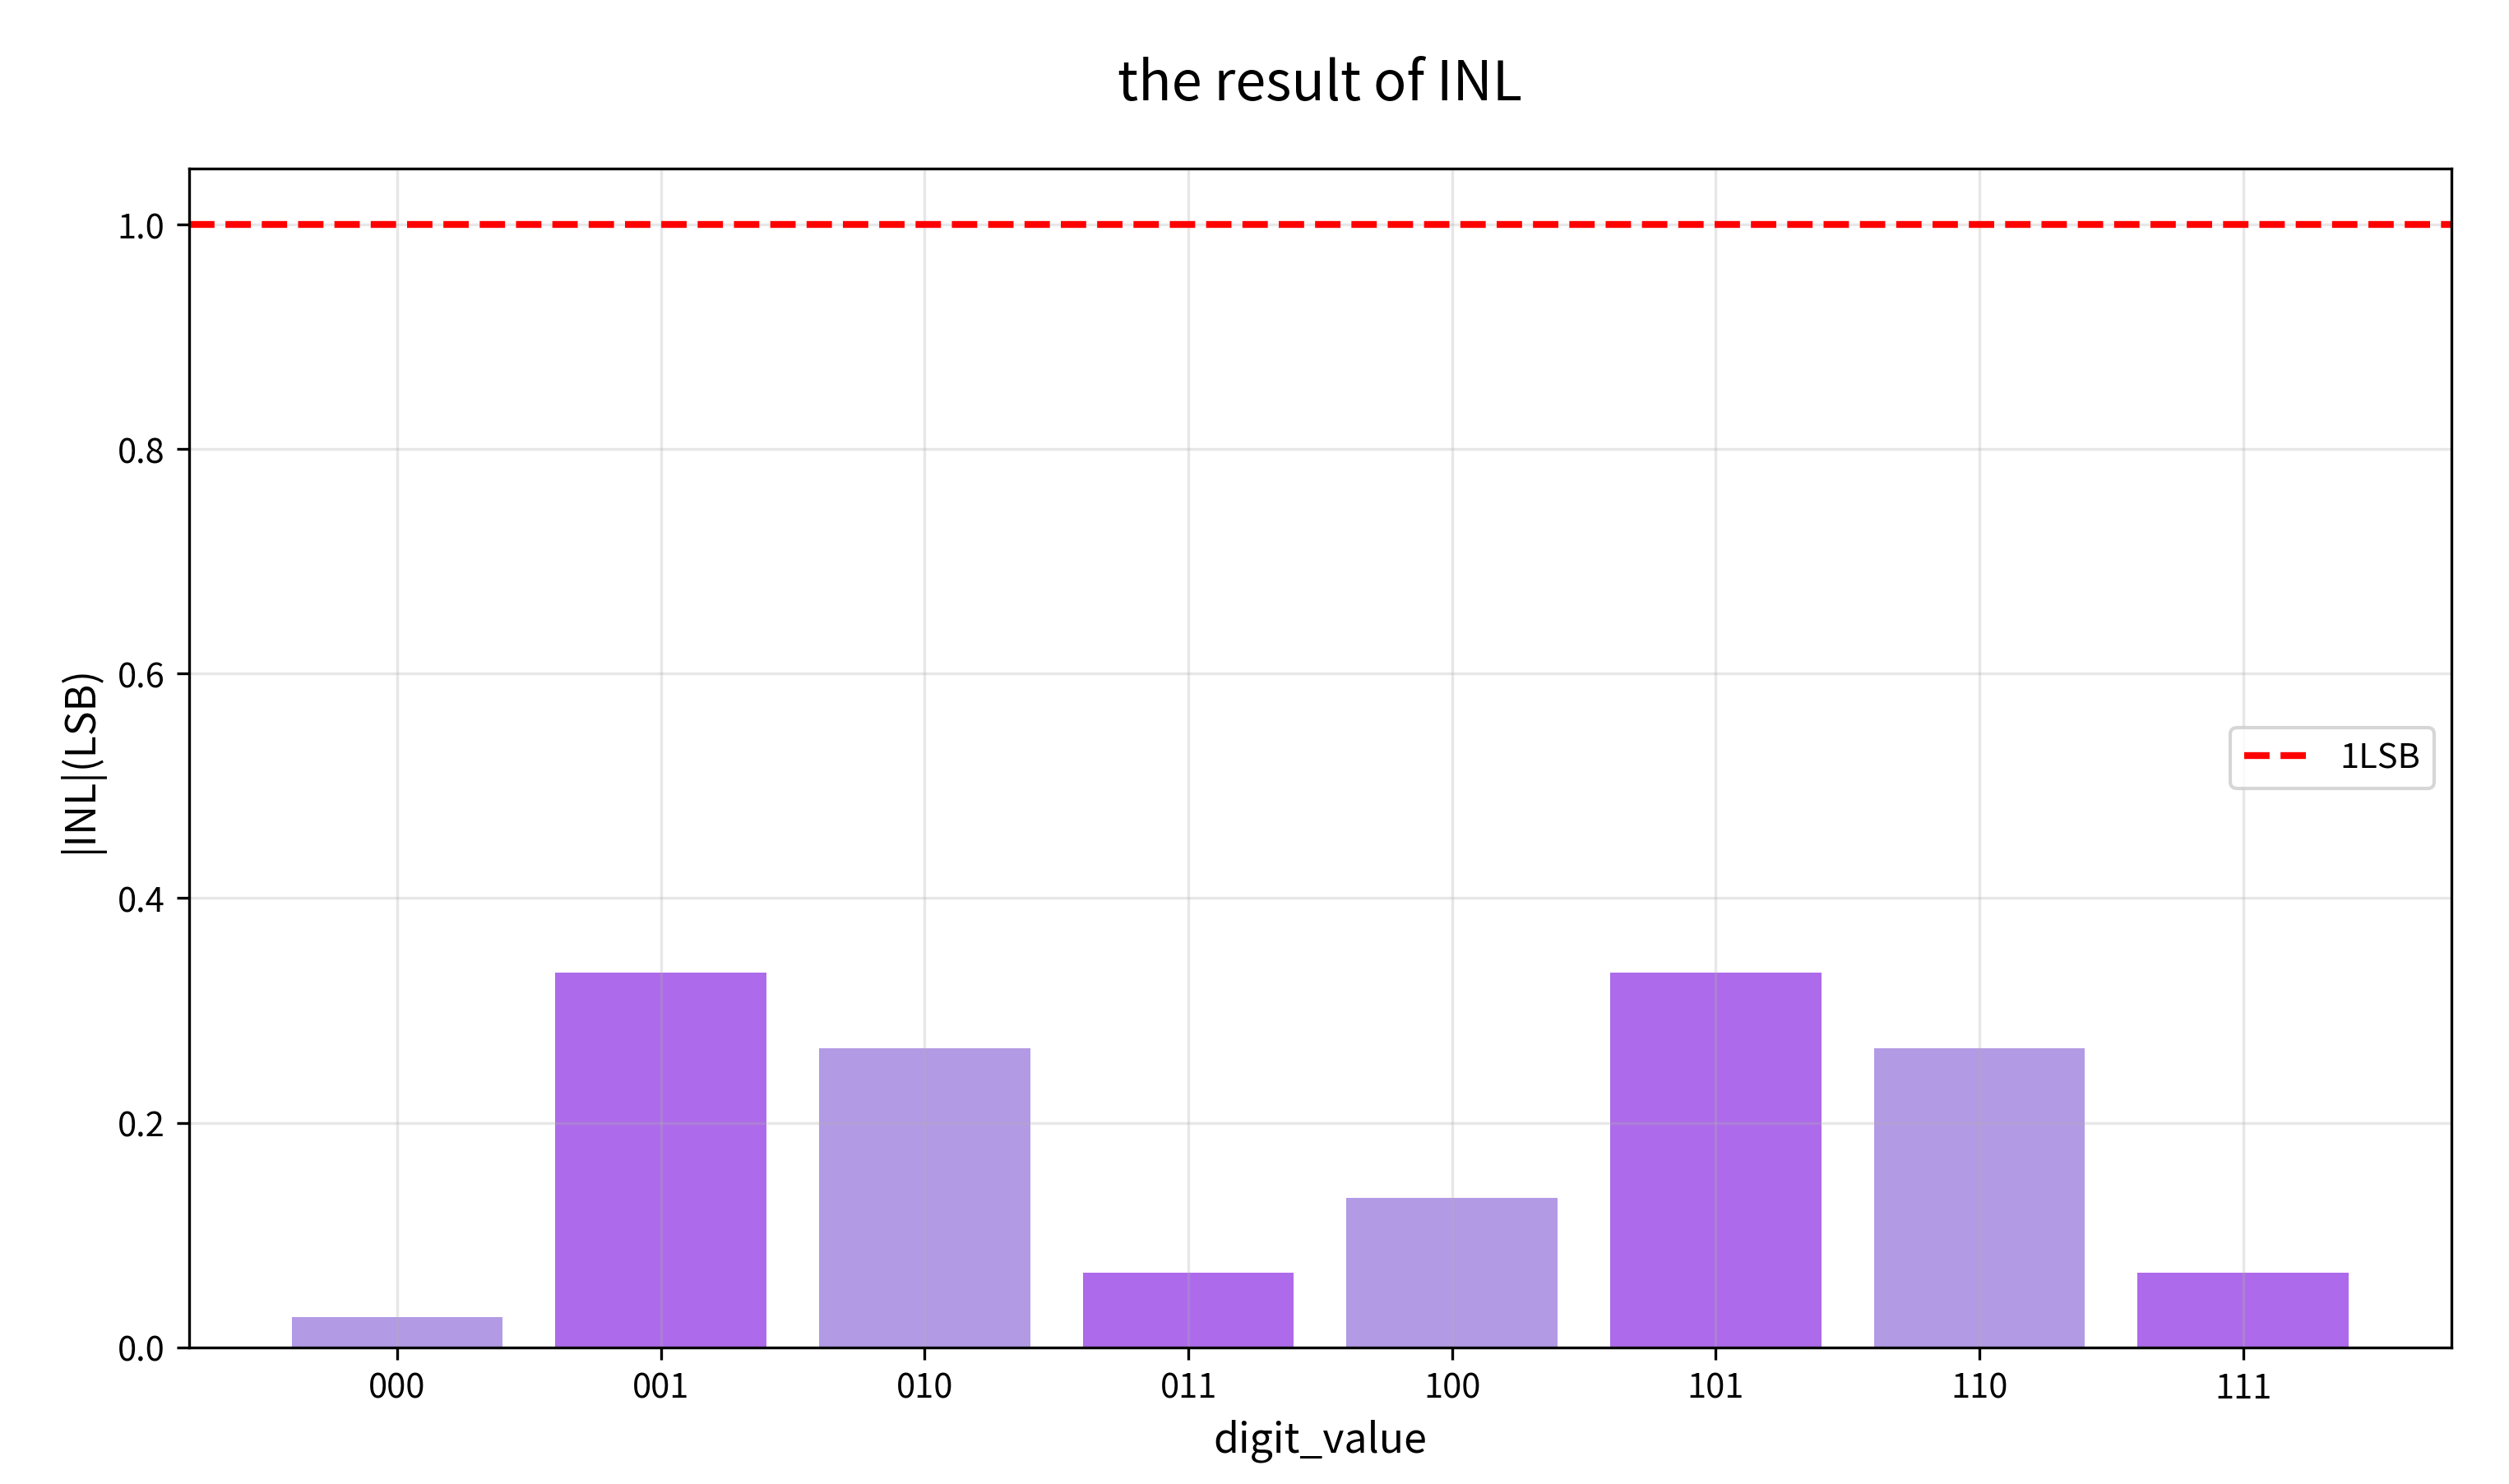
\includegraphics[width=0.48\textwidth]{the result 3 INL.png}}
\caption{Bar Chart of INL}
\label{fig}
\end{figure}

\subsection{Error Analysis}  
  
As shown in Table \ref{tab1} and Figs. 19 and 20. It is crucial to acknowledge that these results represent the theoretical performance limit of the designed architecture. In the simulation environment, the passive components (the $R$ and $2R$ resistors in the ladder network) were assigned exact values, and the active devices (MOSFETs in switches and the OTA) were modeled with perfect matching parameters.  
  
In a practical semiconductor fabrication process, however, non-ideal characteristics and component mismatches are inevitable, which will degrade the DNL and INL performance significantly compared to ideal simulation results. The primary sources of error in a physical implementation of the circuit shown in Fig. 12 are analyzed below:  
  
\subsubsection{R-2R Ladder Resistor Mismatch}  
The fundamental operating principle of the R-2R DAC relies on precise current division, which dictates that the resistance looking into any node must be exactly $2R$. In reality, variations in manufacturing processes (such as doping concentration gradients or etching inaccuracies) lead to mismatches between individual resistor units.  
  
In the circuit of Fig. 12, deviations in the precise ratio between the longitudinal $R$resistors. Mismatch in the most significant bit (MSB) resistors has the most severe impact on DNL, particularly at the major carry transition (e.g., from code 011 to 100), potentially causing non-monotonic behavior if the errors exceed \SI{1}{LSB}. The cumulative effect of these resistor mismatches across the entire ladder directly contributes to the global INL error.  
  
\subsubsection{Switch Non-Idealities and Mismatch}  
The NMOS transistor pairs used as switches in the input stage (Fig. 12) introduce errors through finite on-resistance ($R_{on}$) and device mismatch.  
\begin{itemize}  
    \item \textbf{Finite $R_{on}$ Effect:} Ideally, the switches would have zero resistance when ON. In practice, they add a finite resistance in series with the $2R$ branch resistors. Although large ladder resistor values (R=$\SI{1}{\mega\ohm})$ were selected in this design to minimize the relative impact of $R_{on}$, it cannot be entirely eliminated, leading to gain error and slight linearity degradation depending on the voltage across the switch.  
    \item \textbf{$R_{on}$ Mismatch:} More critically, process variations in threshold voltage ($V_{th}$) and dimensions ($W/L$) across the die result in different $R_{on}$ values for switches in different bit branches. This $R_{on}$ mismatch disrupts the precise R-2R ratio, contributing to localized DNL errors similar to resistor mismatch.  
\end{itemize}  
  

\section{Conclusion}

This paper has presented the complete design, implementation, and performance analysis of a 3-bit R-2R ladder Digital-to-Analog Converter (DAC) in a \SI{180}{\nano\meter} CMOS process. The DAC architecture comprises three key components: a complementary transmission gate switch network for digital input control, a precise R-2R resistor ladder for binary-weighted current generation, and a custom-designed five-transistor Operational Transconductance Amplifier (OTA) for current-to-voltage conversion.

The simulation results demonstrate that the implemented DAC achieves excellent linearity performance, with a maximum Differential Nonlinearity (DNL) of \SI{0.31}{LSB} and a maximum Integral Nonlinearity (INL) of \SI{0.33}{LSB}. These values are well within the critical thresholds of \SI{0.5}{LSB} for DNL and \SI{1}{LSB} for INL, guaranteeing monotonic behavior and the absence of missing codes across the entire input range. The OTA core, operating with a \SI{20}{\micro\ampere} bias current, provides a DC gain of \SI{41.5}{\deci\bel} and a bandwidth exceeding \SI{30}{\kilo\hertz}, adequately supporting the DAC's operation.


\begin{thebibliography}{00}
\bibitem{b1} T. C. Carusone, D. A. Johns, and K. W. Martin, Analog Integrated Circuit Design, 2nd ed. Hoboken, NJ, USA: John Wiley \& Sons, 2011, pp.445--472.
\end{thebibliography}

\end{document}
